\documentclass[11.5pt,twocolumn]{article}
\setlength{\columnsep}{1cm}
\usepackage[a4paper,hmargin=2cm,vmargin=2.5cm]{geometry}

%! ROOT=adventure.tex
\usepackage{array}
\usepackage{url}
\usepackage{dirtytalk}
\usepackage{graphicx}
\usepackage{lmodern}
\usepackage{mdframed}
\usepackage{xcolor}
\usepackage{xspace}

\newcommand\bodhran{Bodhr\'{a}n\xspace}
\newcommand{\pngname}[1]{\underline{\textit{\textsc{#1}}}}
\newcommand{\npcname}[1]{\underline{\textit{\textsc{#1}}}}
\newcommand{\tiro}[2]{tiro \textbf{#1} a difficolt\`{a} \textbf{#2}}

\newmdenv[linecolor=red,backgroundcolor=yellow!25]{infobox}
\newmdenv[linecolor=red,backgroundcolor=cyan!15]{dreambox}
\newmdenv[linecolor=red,backgroundcolor=red!15]{monsterbox}

\newcommand{\dvstat}[5]{
\textbf{DV}: #1 \\
\emph{1 DV}: #2 \\
\emph{2 DV}: #3 \\
\emph{3 DV}: #4 \\
\emph{Punti Vita}: #5 \\
}

\newcommand{\equip}[2]{
\emph{Armi}: #1 \\
\emph{Armatura}: #2 \\
}

\newcommand{\specialstat}[2]{
\emph{Abilit\`{a} Speciali}: #1 \\
\emph{Poteri Magici}: #2 \\
}

\newcommand{\npc}[2]{
\begin{infobox}
\begin{center}
\npcname{#1}
\end{center}
#2
\end{infobox}
}

\newcommand{\monster}[2]{
\begin{figure}[tb]
\begin{monsterbox}
\begin{center}
\npcname{#1}
\end{center}
#2
\end{monsterbox}
\end{figure}
}

\newcommand{\dream}[2]{
\begin{figure}[tb]
\begin{dreambox}
\begin{center}
\textbf{SOGNO:\\
\underline{#1}
}
\end{center}
#2
\end{dreambox}
\end{figure}
}

\newcommand{\object}[2]{
\begin{figure}[tb]
\begin{infobox}
\begin{center}
\textsc{#1}
\end{center}
#2
\end{infobox}
\end{figure}
}



\begin{document}

\title{Orgoglio Ritrovato -- Una Avventura di Lex Arcana}

\author{Stefano Cherubin}
\date{}

\maketitle

%%%%%%%%%%%%%%%%%%%%%%%%%%%%%%%%%%%%%%%%%%%%%%%%%%%%%%%%%%%%%%%%%%%%%%%%%%%%%%%
\section*{Introduzione per i Giocatori}
\`{E} un periodo di intensa attivit\`{a} arcana nella provincia di Britannia, e il governatore ha richiesto l'aiuto del vostro contubernium per verificare dei rapporti di strani fenomeni che giungono dal Vallo.
Un susseguirsi irregolare di incendi, alluvioni, e smottamenti sta oltraggiando i lavori di rafforzamento ed espansione di un castrum.
Dopo tre mesi di continue lamentele delle autorit\`{a} locali, il governatore ha interpellato gli dei tramite un augure.
A quanto pare, una o pi\`{u} delle divinit\`{a} del Pantheon di Roma si oppone ai lavori.
Purtroppo l'augure non \`{e} pi\`{u} in Britannia, in quanto la sua presenza \`{e} stata urgentemente richiesta altrove, ma la preoccupazione rimane.
Il governatore vi chiede di recarvi direttamente ad Eburacum, dove sarete istruiti sui fatti dalle autorit\`{a} locali.

%%%%%%%%%%%%%%%%%%%%%%%%%%%%%%%%%%%%%%%%%%%%%%%%%%%%%%%%%%%%%%%%%%%%%%%%%%%%%%%
\section*{Introduzione per il Demiurgo}
La Legio IX Hispana scomparve nell'anno 873 aUc (Ab Urbe Condita).
Siamo nell'anno 1229 aUc.
Ad oltre 350 anni dalla scomparsa della IX, dal nulla iniziano a riemergere indizi che potrebbero svelare la sorte della Legione perduta.
I lavori di ampliamento del castrum coprono il campo dove la Legio Hispana inizi\`{o} a combattere prima di misteriosamente svanire nel nulla.
La battaglia non \`{e} mai terminata, e Marte ritiene sacro questo terreno fino a che esso non decreti un vincitore di questa battaglia.
I custodes sono chiamati ad indagare su quello che si riveler\`{a} essere uno dei pi\`{u} grandi misteri irrisolti nella storia dell'Impero.
Essi stessi potrebbero ritrovarsi coinvolti in uno scontro con potenze sovrannaturali, uno scontro rimasto in sospeso da pi\`{u} di tre secoli.

%%%%%%%%%%%%%%%%%%%%%%%%%%%%%%%%%%%%%%%%%%%%%%%%%%%%%%%%%%%%%%%%%%%%%%%%%%%%%%%
\section*{Sinossi}

\subsection*{Parte I -- Fiamme di Guerra}
%
Incendi inspiegabili devastano il sito in costruzione.
Lungo la strada per Pons Aelius, i custodes incontrano diversi bardi ad ogni taverna, e occasionalmente dei non-morti nelle campagne.
Giunti in citt\`{a}, i custodes trovano danni sparsi dovuti a catastrofi apparentemente disgiunte.
Nel villaggio, imperversano anche dispetti di un Br\`{u}neus, e un pericolo diplomatico dovuto ad un arresto illustre.
Durante il sopralluogo dei custodes, nottetempo uno scirpex infuocato compare dal nulla e incendia alcuni edifici.

\subsection*{Parte II -- Eco dal Passato}
Il campo di battaglia restituisce alcuni corpi, alcuni ancora vivi.
I resti dello scirpex rivelano legionari usati come sacrifici.
Tra loro, compare anche l'effige di un'aquila: quella della Legio IX.
Un misterioso personaggio venuto dal passato si offre di aiutare i custodes nella battaglia contro il culto di Balor.

\subsection*{Parte III -- La Battaglia pi\`{u} Lunga}
Tafferugli con cultisti invasati rallentano il contubernium.
Ispirati da un sogno, i custodes possono ottenere la benedizione delle divinit\`{a} locali del Vallo.
La magia che trattiene i combattenti nel reame fatato collassa e i custodes sono catapultati in un mezzo ad una rivolta di proporzioni mai viste.
La battaglia \`{e} ancora in corso e la Legio IX ha bisogno di assistenza.
Riusciranno i custodes a uscirne vittoriosi?

%%%%%%%%%%%%%%%%%%%%%%%%%%%%%%%%%%%%%%%%%%%%%%%%%%%%%%%%%%%%%%%%%%%%%%%%%%%%%%%
\subsection*{Valore indicativo}
Punti Esperienza: 8

%%%%%%%%%%%%%%%%%%%%%%%%%%%%%%%%%%%%%%%%%%%%%%%%%%%%%%%%%%%%%%%%%%%%%%%%%%%%%%%
%\clearpage
\section*{Luoghi}
\begin{description}
\item[Eburacum] Capoluogo della Britannia Quarta (o Ultima). Qui i custodes vengono convocati e aggiornati sui fatti dal governatore. \\Toponimo moderno: York.
\item[Pons Aelius] Castrum sul limes settentrionale collegato al Vallo di Adriano. Qui i custodes vengono incaricati di raccogliere informazioni da testimoni diretti. \\Toponimo moderno: Newcastle Upon Tyne.
\item[Vercovicium] Castrum sul limes posizionato circa a met\`{a} del Vallo. Dista circa 12~h di marcia da Pons Aelius. Vi \`{e} un tempio di Marte in cui si venerano anche le dee britanniche Alaisiagae.
\item[Segedunum] Anche detto \emph{Finis Valli}, \`{e} il forte pi\`{u} a est del Vallo e guarda la foce del fiume Tina. Contiene abitazioni civili dentro le mura, e un piccolo porto fluviale.
\end{description}

%%%%%%%%%%%%%%%%%%%%%%%%%%%%%%%%%%%%%%%%%%%%%%%%%%%%%%%%%%%%%%%%%%%%%%%%%%%%%%%
\section*{Personaggi}
%
\npc{Sextus Domitius Mircianus}{
\dvstat{8}
{Sensibilitas}
{De Bello, De Corpore, De Natura (Cavalcare), Ratio, Punti Vita}
{De Societate (Politica, Negoziare), De Bello (Tattica)}
{16}
Governatore della provincia di Britannia.
Contrariamente alla tradizione di appuntare non nativi al governo di una provincia, egli \`{e} autoctono.
Ha giurato fedelt\`{a} all'imperatore, ma mantiene alcuni usi e tradizioni di origine non romana.
Questa inusuale combinazione sembra essere un fattore determinante nel tenere a bada le insurrezioni locali, anche se a fatica.
Si mormora che tra i suoi assistenti si nascondano dei druidi.
Maggiori informazioni sono disponibili a pagina 25 del manuale Britannia~\cite{britannia_en}.

Ha convocato la corte arcana perch\'{e}, oltre ai rapporti ricevuti, uno dei suoi consiglieri druidi ha confermato la natura sovrannaturale degli eventi a Pons Aelium.
In cuor suo, spera che il suo consigliere si sbagli, ma la posta in gioco \`{e} troppo importante per non verificare.
Sa che ammettere di avere druidi al suo servizio porterebbe alla sua rimozione dall'incarico, nel migliore dei casi.
}

\vfill

\npc{Publius Aurelianus Constans}{
\dvstat{8}
{Sensibilitas}
{De Bello, De Corpore, De Natura (Cavalcare), Ratio, Punti Vita}
{De Societate (Politica, Negoziare), De Bello (Tattica)}
{16}
Legato della Britannia Ultima e cugino dell'imperatore Teodomiro da parte di madre.
Ha la sua sede ad Eburacum e si gode la vita di citt\`{a} ai confini dell'impero, ma visita spesso i castra lungo il vallo.
Quando i custodes arrivano ad Eburacum, egli sta ancora circolando tra i castra sul limes.
\`{E} un politico e generale capace ed efficace.
Fornir\`{a} ai custodes piena collaborazione, anche se sue uniche esperienze con il soprannaturale si limitano a combattere sporadici cadavera turbari.
Maggiori informazioni sono disponibili a pagina 56 del manuale Britannia~\cite{britannia_en}.
}

\eject

\npc{Ellfin Pupius}{
\dvstat{8}
{De Bello, De Corpore}
{Punti Vita, De Natura, De Scientia}
{De Societate, De Magia (Disciplina Druidiica)}
{16}
Assistente e consigliere personale di Sextus Domitius Mircianus.
Nativo della Britannia Quarta, \`{e} considerato un ``nuovo romano''.
Il suo status sociale dipende dal governatore, ed a lui \`{e} rivolta la sua fedelt\`{a}.
Il suo lavoro richiede di mantenere contatti con le trib\`{u} native dell'isola, dentro e fuori i confini imperiali.
Ha una discreta conoscenza della lingua e cultura locale.
Si mormora che sia un druido in incognito.
}


\npc{Il Musico Bicentenario}{
\dvstat{6}
{De Bello, De Scientia}
{Punti Vita, De Natura, De Corpore}
{De Societate, De Magia}
{12}
\begin{center}
\vspace{-2.5em}
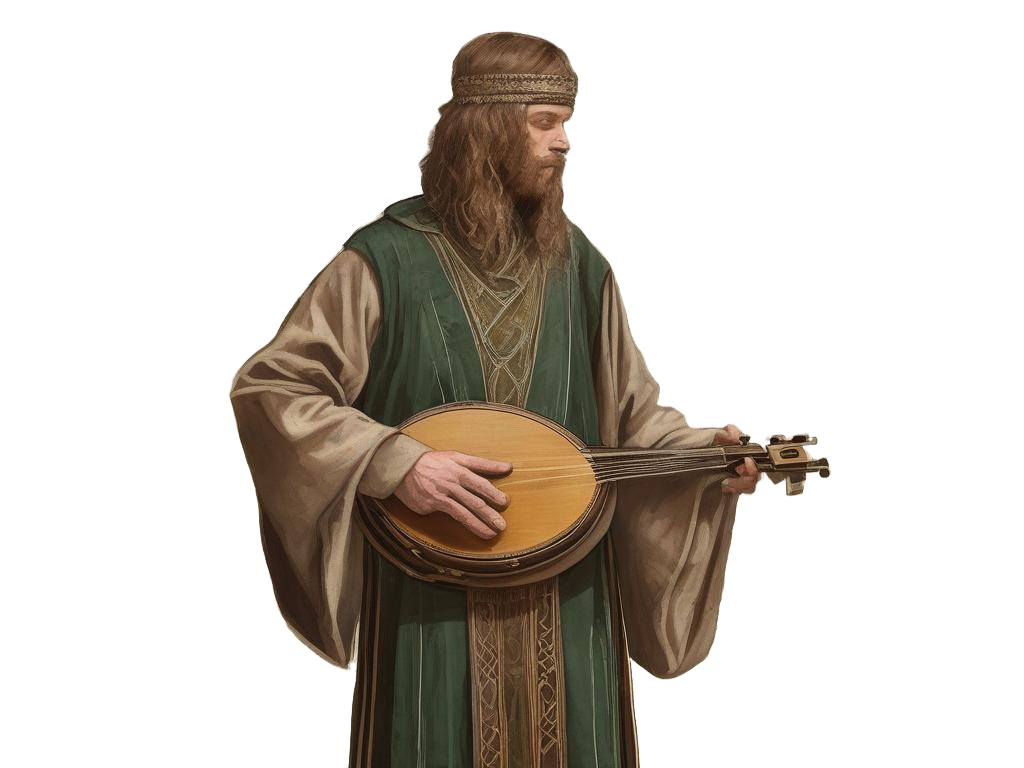
\includegraphics[width=.65\columnwidth]{img/musico.png}
\vspace{-1em}
\end{center}
Appare come un uomo robusto e trasandato dall'aspetto di circa venticinque anni.
Da circa due anni vive come musico itinerante nelle taverne della Britannia Quarta.
In vero, egli davvero nacque pi\`{u} di due secoli fa, ma esita a raccontare in giro questa verit\`{a} per timore di passare per matto.
Usa il nome di musico bicentenario come nome d'arte.
Racconta la sua vera storia solo attraverso le sue canzoni, o a gente troppo ubriaca per prenderlo sul serio.

Egli venne risucchiato nella terra senza tempo dalla Parva Gens mentre suonava il flauto sulla riva di un ruscello nella foresta.
Non sa come lui abbia attraversato la barriera tra il nostro mondo e quello della parva gens, ma sospetta che lo abbiano lasciato andare solo quando smise di suonare il flauto e inizi\`{o} a padroneggiare le percussioni.
Ha ripreso conoscenza in una taverna vicino al limes due anni fa, vestito di stracci e accompagnato solo dal suo flauto e dal suo \bodhran (tamburo celtico).
Da allora suona soltanto il suo \bodhran e ha il terrore del suono dei flauti.

La sua musica ha davvero un effetto sulla Parva Gens, ma lui sembra non avere bene idea di come controllare questo potere.
}


\npc{Sp\`{o}g Nan Sionnach}{
\dvstat{10}
{De Bello, Sensibilitas}
{De Scientia, De Corpore, De Societate, Punti Vita}
{De Natura, De Magia (Disciplina druidica)}
{20}
%\begin{center}
%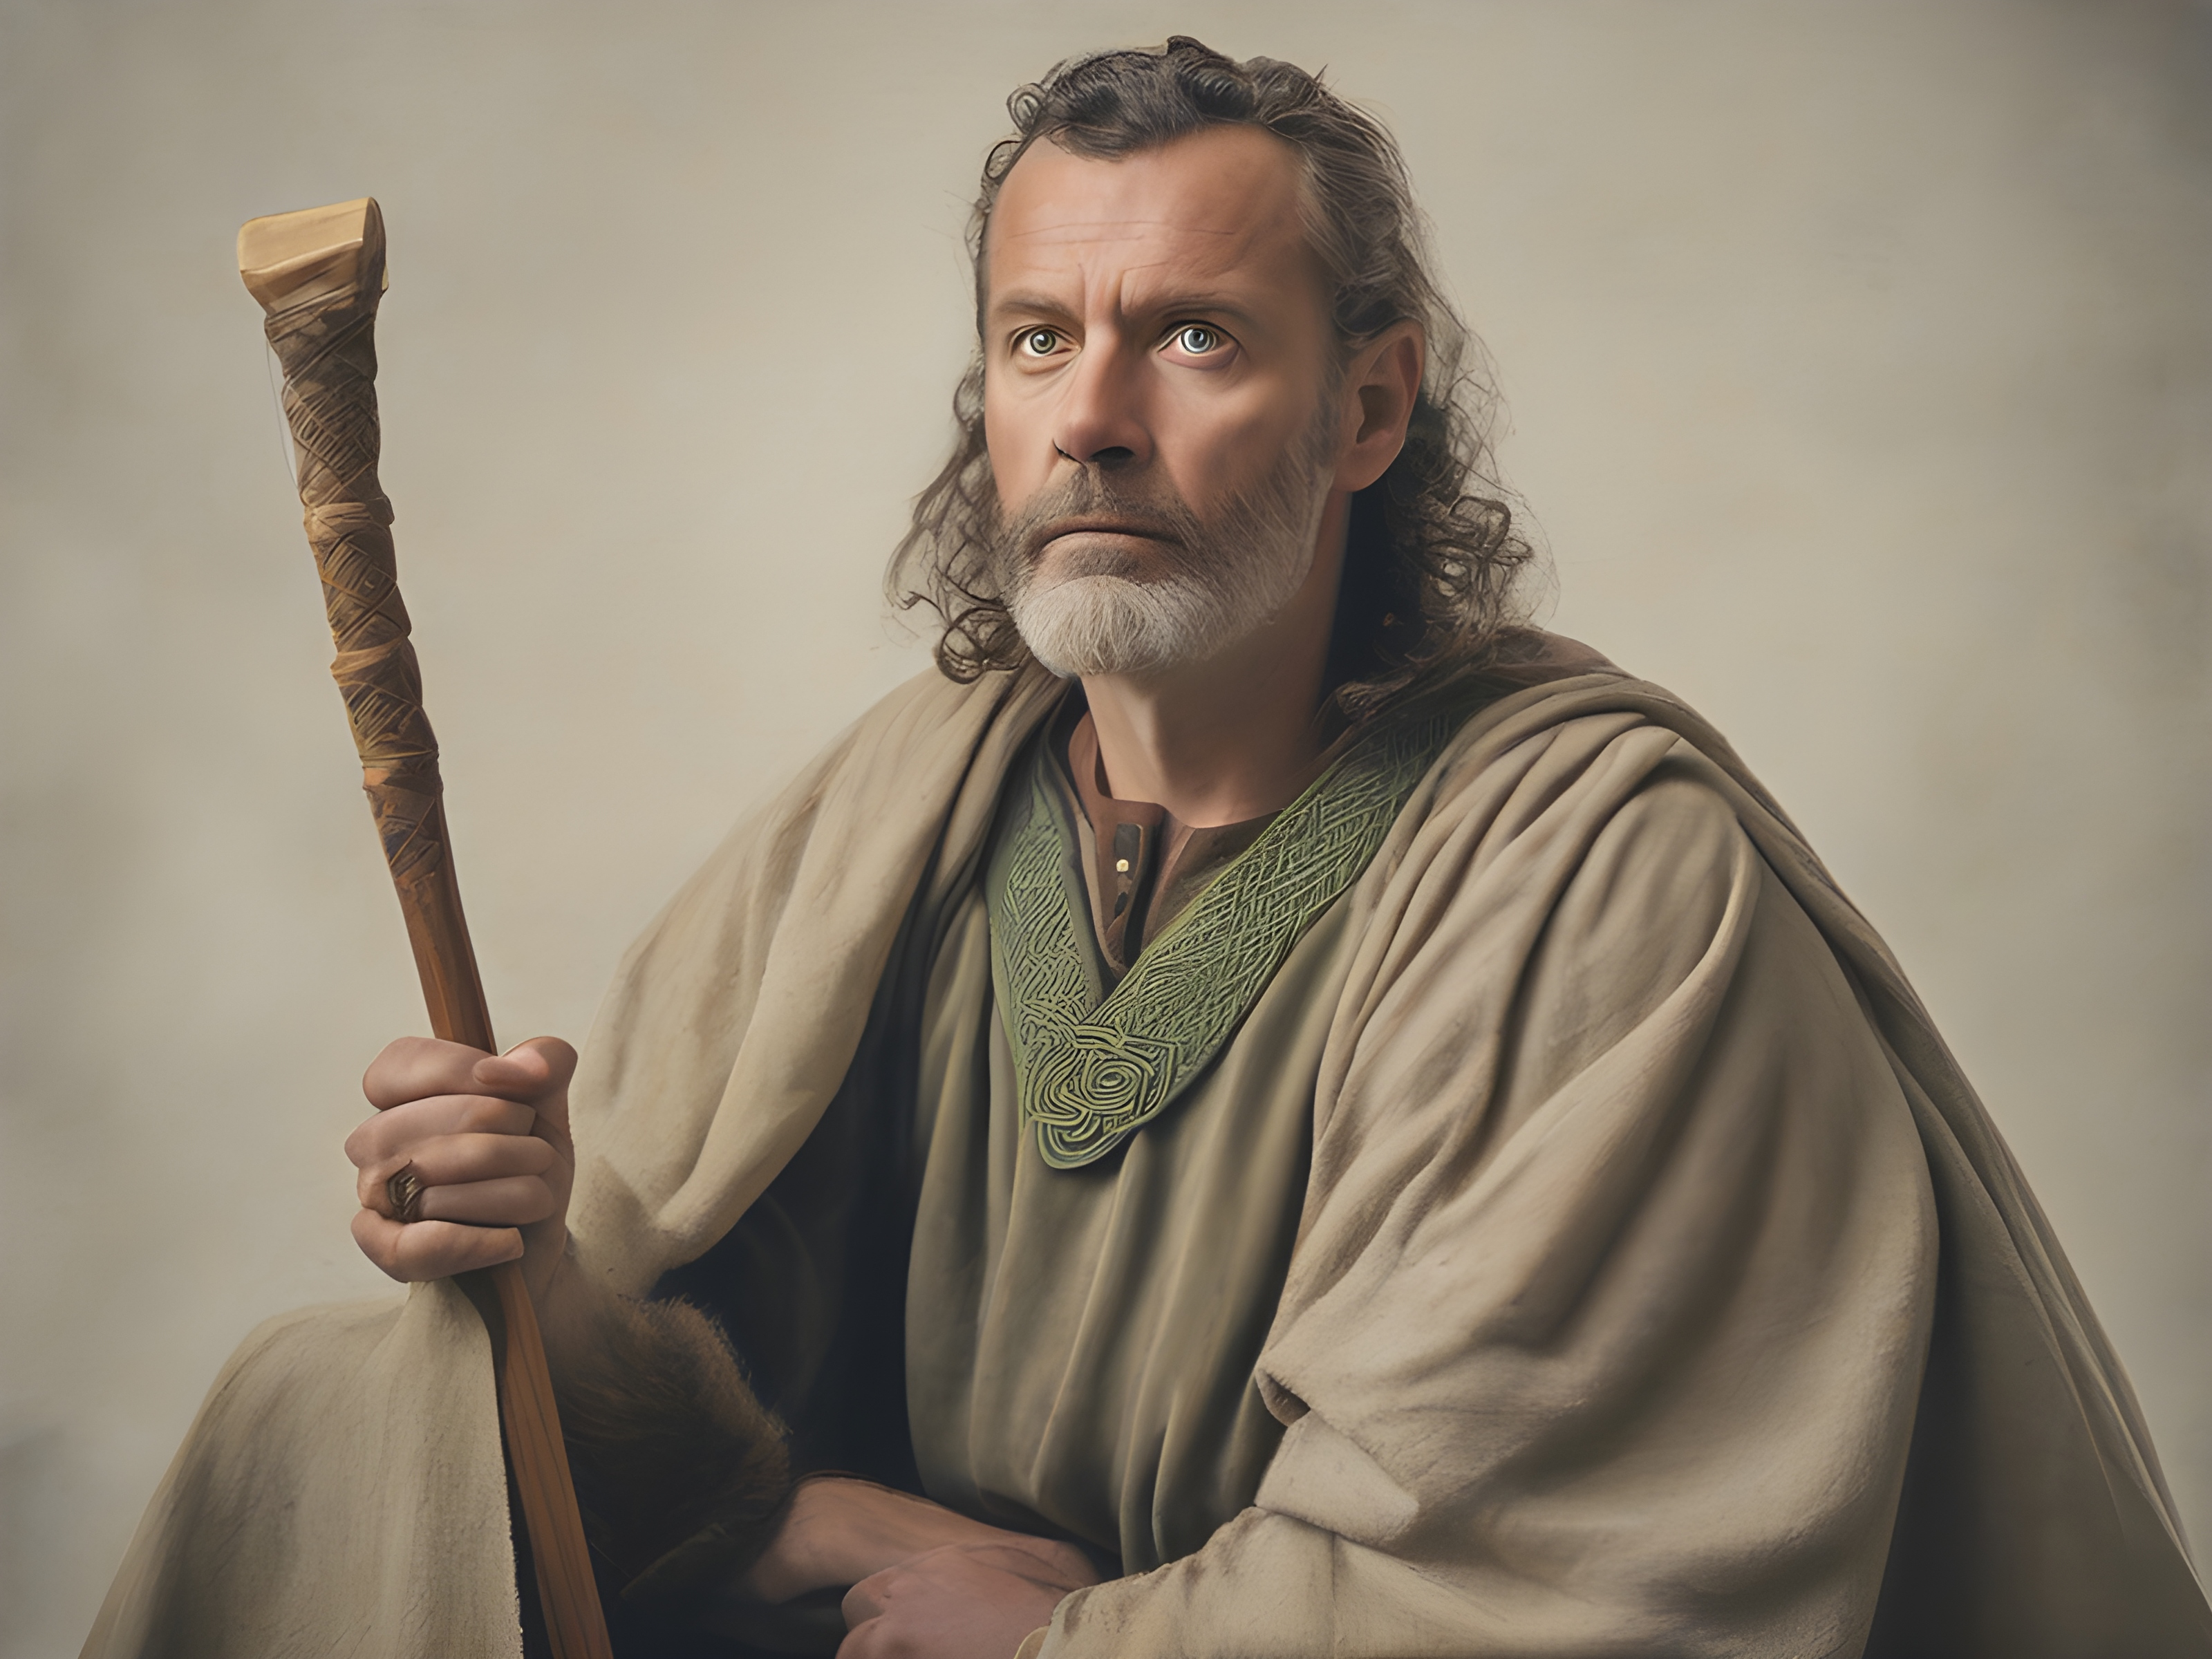
\includegraphics[width=\columnwidth]{img/arcidruido.jpeg}
%\end{center}
Nel 873 aUc ricopriva il ruolo di Arcidruido.
Il suo nome significa ``zampa di volpe''.
\`{E} un uomo di circa quarant'anni, dai capelli brizzolati e dal busto molto esile.
Braccia e gambe, al contrario sono molto muscolose.

Quando venne a sapere dei piani dell'antico arcivate per portare l'ira di Balor in Britannia, si organizz\`{o} con la Parva Gens per bloccare il suo esercito in un mondo parallelo, in un remoto angolo del reame fatato in cui il tempo scorre diversamente.

Non \`{e} amico di Roma, ma vede l'impero come ultima risorsa per fermare l'avvento di Balor.
}


\npc{Cluas a' Ge\`{a}rra}{
\dvstat{8}
{De Bello, Sensibilitas}
{De Natura, De Scientia (Storia), De Corpore, Punti Vita}
{De Societate (Intrattenimento), De Magia (Disciplina druidica)}
{16}
\begin{center}
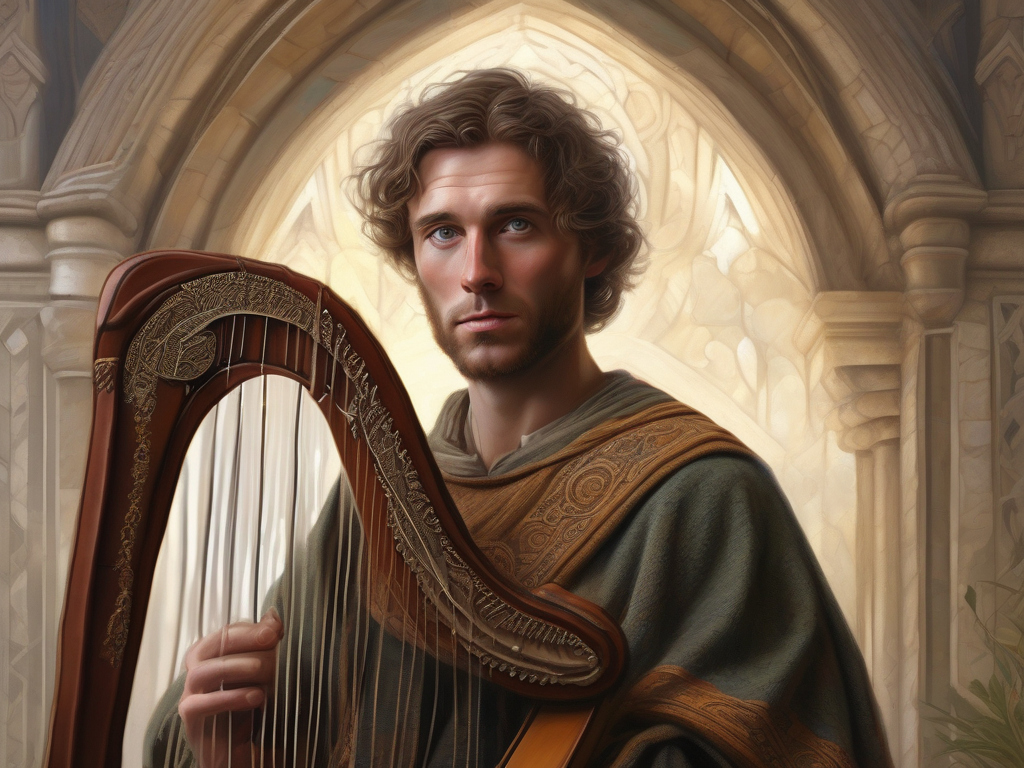
\includegraphics[width=\columnwidth]{img/bardo.jpeg}
\end{center}
Nel 873 aUc ricopriva il ruolo di Arcibardo.
Il suo nome significa ``orecchio di lepre''.

Si alle\`{o} con Sp\`{o}g per combattere contro l'arcivate corrotto da Balor ma rimase intrappolato nel reame fatato.

Conosce a memoria le antiche leggende di tutta la Britannia e di buona parte di Hibernia.
}

\npc{Georgius Mar Mathan}{
\dvstat{8}
{Ratio, De Scientia, De Magia}
{De Bello, De Societate, Punti Vita}
{De Natura (Cacciare), De Corpore (Lotta)}
{16}

Ex minatore di etnia brigante dal fisico molto robusto ma dal volto ancora sbarbato.
\`{E} promesso sposo alla primogenita di un importante capo trib\`{u} locale.
Dopo la chiusura della miniera, si \`{e} dato alla caccia di frodo rubando sei cervi dalla riserva caccia privata dell'imperatore Teodomiro.
I legionari del castrum lo hanno arrestato al mercato pochi giorni prima dell'arrivo dei custodes mentre cercava di vendere la selvaggina rubata vantandosi del misfatto.
\`{E} stato condannato all'impiccagione, ma le trib\`{u} locali potrebbero scatenare una rivolta se questa sentenza venisse eseguita.
}


\npc{Quinto Petilio Ceriale}{
Petilio fu un donnaiolo, un politico, e un capace condottiero.
Ha sedato molte rivolte come capo della Legio IX Hispana in varie province sul limes.
In particolare, si concentr\`{o} nelle province Britannia Secunda e Britannia Quarta.
\`{E} il fondatore della urbe fortificata Eburacum, oggi capitale della Britannia Quarta.
Non segu\`{i} la Legio IX nella battaglia in cui scomparve. Per la disfatta riportata, la sua carriera politica ne risent\`{i} molto, ma riusc\`{i} comunque ad essere promosso senatore, prima di morire di vecchiaia nella sua villa di Roma Urbe.
}


%%%%%%%%%%%%%%%%%%%%%%%%%%%%%%%%%%%%%%%%%%%%%%%%%%%%%%%%%%%%%%%%%%%%%%%%%%%%%%%
\section*{Fatti antecedenti}
Nell'anno 873 aUc, l'Arcivate di Britannia ed Hibernia guid\`{o} una rivolta contro Roma.
Nel tentativo di sopraffare la superiorit\`{a} militare dell'Impero, egli speriment\`{o} una combinazione di magia druidica, culto di Agrona\footnote{Vedi manuale Britannia~\cite{britannia_en} a pagina 106.}, e culti fomoriani meno conosciuti.
In particolare, venne corrotto dal culto del dio fomoriano della distruzione Balor.\footnote{Vedi manuale Britannia~\cite{britannia_en} a pagina 109.}

Inizialmente suoi alleati, temendo la distruzione di ogni civilt\`{a} umana conosciuta, l'Arcibardo e l'Arcidruido del tempo gli si rivoltarono contro quando l'Arcivate inizi\`{o} ad evocare l'Emissario di Balor.
Arcibardo ed Arcidruido iniziarono quindi un rituale per bloccare l'Arcivate, il suo esercito, ed i suoi scirpex in un angolo remoto del reame fatato, dove il tempo scorre pi\`{u} lentamente.

La Legio IX ingaggi\`{o} i rivoltosi in una difficile battaglia, nel mezzo della quale il rituale per fermare il tempo venne innescato.
Ora la Legio IX sta combattendo contro l'Arcivate ed il suo intero esercito formato da Pitti, Caledoni, Briganti, ed altre trib\`{u} minori nemiche di Roma.
Larghe buche nascoste nel terreno portano i legionari a venire prima intrappolati e subito dopo sacrificati per far nascere Scirpex di Balor, golem sotto il controllo dell'Arcivate.
Bloccati in un limbo del reame fatato dove un giorno equivale a 500 anni nell'impero, la battaglia non \`{e} ancora terminata.

I lavori di espansione del castrum stanno interferendo con i cerchi sacri che hanno posto l'antico Arcidruido e l'antico Arcibardo nelle vicine miniere di Antimonium (allora conosciuto con il nome di \emph{Stibium}).
Il crollo di una vecchia miniera ha causato il disallineamento delle ghiande sacre del rituale, il quale sta perdendo efficacia.
Poco alla volta, gli eserciti stanno uscendo dal reame fatato.

Le cronache ufficiali riportano meno informazioni circa la Legio IX, vedere box a pagina 17 del volume Britannia~\cite{britannia_en}.

%%%%%%%%%%%%%%%%%%%%%%%%%%%%%%%%%%%%%%%%%%%%%%%%%%%%%%%%%%%%%%%%%%%%%%%%%%%%%%%
\section*{Parte I -- Fiamme di Guerra}

\subsection*{Scena I\\Incaricati di Non Trovare Nulla}
%
La lettera di convocazione per l'incarico giunge da Londinium e riporta il sigillo del governatore Sextus Domitius Mircianus (Vedi manuale Britannia~\cite{britannia_en} -- pagina 25 per approfondimenti).
I custodes sono convocati direttamente ad Eburacum, non a Londinium.
Questa prassi \`{e} inusuale per molte province, ma non per la Britannia.
In questa provincia, \`{e} normale per il governatore visitare molto spesso le diverse regioni in cui la Britannia \`{e} suddivisa.
Sextus Domitius riceve i custodes ed illustra loro il problema.

S.D.M. -- \say{%
Custodes, il limes non \`{e} mai stata l'area pi\`{u} tranquilla dell'impero e mi giungono spesso lamentele dai soldati di istanza sul Vallo o nella Britannia Ultima.
Pare che ci siano inspiegabili eventi di sabotaggio in quel di Pons Aelium.
Stiamo cercando di ampliare il castrum e rendere l'accampamento pi\`{u} accogliente per i soldati e le loro famiglie.
Potrebbe essere qualche trib\`{u} di Caledoni che si oppone all'ampliamento, ma mi sembra strano: il grosso dei lavori riguarda migliorie delle strade, e nuove botteghe.
Niente di militare
}\\
Ellfin Pupius -- \say{%
Mircianus, forse sarebbe il caso di parlare dei presagi
}\\
S.D.M. -- \say{%
Oh, giusto! Grazie, me ne stavo per scordare.
Allora, un paio di settimane fa stavo per cestinare l'ennesima lettera di lamentele, quando un cattivo presagio ha rovesciato la candela e incendiato mezzo scrittoio.
Questo mi ha fatto pensare e ho interpellato i miei assistenti, ed abbiamo richiesto la consulenza di un augure... -- sospira -- gente rara di questi tempi gli auguri!
Insomma, uno tra gli dei -- non sappiamo quale -- si oppone persino alla costruzione di un tempio romano!
Qualcosa non torna.
Mi piacerebbe che andaste a fare un sopralluogo e tornaste dicendo che l'augure si \`{e} sbagliato.
O che hanno sbagliato a fare un capitello.
O che la pittura era marcia e Apollo si \`{e} offeso per quello
}

S.D.M. conversa con i custodes per circa un'ora e risponde ad eventuali domande che loro possano avere.
Prima di partire per una importante occasione mondana nella Britannia Secunda, si sincera che abbiano sufficienti conoscenze della lingua e delle tradizioni locali.
Dovessero i custodes chiedere ulteriore assistenza, SDM lascia uno dei suoi assistenti in compagnia dei custodes: Ellfin Pupius.


\subsection*{Scena II\\Gatti, Pecore, e Torbiere}
%
\monster{Minio Matholwch}{
\dvstat{6}
{Danno, De Bello, Ratio}
{De Corpore, Sensibilitas, Punti Vita}
{De Scientia (Enigmi), De Magia}
{12}
\specialstat{Velocit\`{a} innaturale}
{Mutaforma}
Questo fatuo ha scelto di dimorare nella locanda di Pons Aelium e la protegge con la sua magia finch\'{e} vi risiede.
Occasionalmente vaga per villaggi vicini sotto forma di gatto selvatico.
Torna sempre alla taverna dove sa di trovare una porzione di zuppa di pane e un boccale di birra lasciate da un vecchio servitore con il potere dei \emph{Tint\`{i}nni}.
Quando il servitore non \`{e} di turno, o per qualunque motivo non lascia doni, Minio lancia uno dei suoi dispetti sugli avventori.
Il suo dispetto preferito \`{e} far marcire la birra appena spillata nei boccali.

Minio appartiene alla razza Br\`{u}nei dei fatui clari. Vedi manuale Britannia~\cite{britannia_en} a pagina 178.

Vedi manuale Britannia~\cite{britannia_en} a pagina 125 per i fatui clari; a pagina 164 per i Tint\`{i}nni.
}
%
Il viaggio verso Pons Aelius \`{e} inizialmente privo di problemi.
Lungo la via, ville e locande gestite da romani avranno problemi di birra inspiegabilmente andata a male da un giorno all'altro.
%
Occasionalmente, i custodes pi\`{u} attenti (\tiro{Sensibilitas}{9}) noteranno altre piccole cose fuori posto in queste locande.
%
Un custos eccezionalmente attento (\tiro{Sensibilitas}{12}) avr\`{a} una sensazione di qualcosa di magico nel locale e pu\`{o} accorgersi di un grosso gatto selvatico che sonnecchia in un angolo o sopra una trave, accanto ad uno o due altri gatti domestici.
Si tratta di Minio Matholwch.
Non sar\`{a} possibile catturare Minio in alcun modo prima dell'arrivo a Pons Aelius.

Se decidono di fermarsi in una locanda, i custodes incontrano il Musico Bicentenario, il quale riscuote discreto successo tra gli avventori. Quando si accorge della presenza di legionari, il musico cerca di evitare di attirare l'attenzione su di s\'{e} e canta solo in lingua celtica.

\monster{Cadaver Turbari}{
\dvstat{6}
{Danno, Sensibilitas}
{De Bello, De Corpore, Ratio}
{De Corpore (Lotta), Punti Vita}
{18}
\specialstat{Afferrare, Furtivo*}
{Ferite Permanenti, Immortalit\`{a}, Malattia (2DV, la vittima deve essere ferita dalla creatura), Nebbia}
\emph{* I tiri per individuarli hanno soglia maggiorata di 2 livelli.}\\
\emph{** Se la Malattia porta a 0 i Punti Vita della vittima, questa si trasforma a sua volta in Cadaver Turbarii senza pi\`{u} volont\`{a} propria. La vittima pu\`{o} opporre un tiro Ratio ogni tempus per resistere alla Malattia.}

Vedi manuale Britannia~\cite{britannia_en} a pagina 174 per ulteriori dettagli.
}

Verso met\`{a} del tragitto verso Pons Aelius, i custodes assistono alla seguente scena.
Un pastore corre incontro ai custodes domandando aiuto.
Basta un \tiro{Sensibilitas}{3} per notare fin da lunga distanza che si trova in chiaro stato di agitazione.
Quando si avvicina, egli racconta ai custodes che le sue pecore hanno bevuto dall'acquitrino sbagliato e per sbaglio hanno risvegliato dei mostri.
I custodes potranno scegliere se deviare mezza giornata per aiutarlo o ignorare la sua richiesta.
Nel caso in cui andranno ad aiutarlo, si troveranno a combattere contro dei cadavera turbarii.
Compare un cadaver per ogni 2 custos nel contubernium (arrotondare per eccesso).
Nel caso in cui si rifiuteranno, i cadavera mieteranno altre vittime e il rapporto salir\`{a} a 1:1 quando, poche ore dopo, attaccheranno il contubernium in una imboscata.

\subsection*{Scena III\\Arrivo a Pons Aelius}
%
Pons Aelius \`{e} un castrum militare fortificato sulla riva settentrionale del fiume Tinea\footnote{Talvolta riportato sulle mappe come Vedra. Toponimo moderno: Tyne} e per molti anni ha servito da limite orientale del Vallo di Adriano.
Oggi il vallo prosegue per ulteriori 5 miglia verso oriente, anche se gi\`{a} da Pons Aelius il Tinea \`{e} largo a sufficienza da costituire una buona linea difensiva.
Questo castrum si trova a circa dieci miglia dall'Oceano Germanicus.
Come suggerisce il nome, l'attrazione principale di questo luogo \`{e} un ponte costruito sul fiume.
Tuttavia, non mancano piccole costruzioni e attivit\`{a} commerciali in zona.

Per arrivare a Pons Aelius, i custodes passano su strade quasi deserte.
Occasionalmente incontrano viandanti, prevalentemente romani di origine Brigante\footnote{Vedi manuale Britannia~\cite{britannia_en} pagina 91.}.
Molto pi\`{u} spesso si troveranno di fronte a cervi selvatici, pecore, e -- durante la notte -- qualche volpe.

A sud del ponte sorgono costruzioni sparse: alcune fattorie, una locanda, e una villa.
Quattro sentieri si diramano dietro le colline partendo dalla locanda.
Seguendo tre di questi sentieri si arriva alle miniere abbandonate.
Il quarto porta in cima alla collina pi\`{u} vicina, dove sono in atto dei lavori di costruzione.

\dream{Non disturbare l'intrattenimento di Marte}{
%
Un grande trono si staglia di fronte al sognatore.
Girandogli attorno, si delinea la figura di una donna che vi siede.
Sulla spalla della donna, una colomba bianca siede appollaiata.
Accanto alla donna, siede una figura maschile.
L'uomo \`{e} agitato e brandisce una lancia nella mano destra mentre tiene lo sguardo fisso verso un punto remoto della stanza dove si svolge una piccola baruffa.
Un cucciolo di lupo si sta azzuffando contro un cervo.
Accanto al cervo, dei grossi topi dagli occhi infuocati sono allineati come a proteggergli i fianchi.

L'uomo scuote ripetutamente la lancia per incitare al combattimento, e in particolar modo sembra favorire il lupo.
Nel frattempo, servitori si avvicinano con abbondanti cesta di frutta fresca.
La donna prende un frutto, lo mangia, e ringrazia il servitore con una carezza.
L'uomo reagisce stizzito quando un servitore gli passa di fronte e gli occlude la visuale.
Nel cacciare via il servitore, la frutta cade a terra.
}


\subsection*{Scena IV\\Le Miniere}
%
Ci sono tre miniere, di cui una chiusa di recente e due abbandonate da molto tempo.
La prima miniera, dislocata a sud-ovest del castrum dista circa 5 miglia e veniva usata per estrarre carbone.
Un editto di Publius Aurelianus ha fatto chiudere la miniera due settimane fa, temendo che la sua attivit\`{a} stesse disturbando gli dei.
La chiusura non ha fermato gli episodi sovrannaturali ma in compenso ha contribuito ad un aumento della disoccupazione locale e del brigantaggio.

La seconda \`{e} una cava di pietra ferrosa 2 miglia a sud di Pons Aelius.
Venne sfruttata molto durante la costruzione del Vallo di Adriano.
Fu chiusa in seguito ad un crollo circa due secoli fa, quando il vallo era gi\`{a} stato terminato.
La sua produzione si era abbassata notevolmente e i suoi costi di ristrutturazione e di mantenimento non erano giustificati dalla rendita.

La terza \`{e} in realt\`{a} una derivazione della seconda miniera, con un ingresso poco pi\`{u} a est.
Qui venne trovato un giacimento di stibium, ora conosciuto come antimonium.
I cristalli di questo minerale erano usati come cosmetico per contornare gli occhi di giovani e ricche bellezze mediterranee.
Questa miniera \`{e} quella chiusa da pi\`{u} tempo e le sue tracce sono oggi a malapena riconoscibili.
Le cause della sua chiusura sono perse nei racconti popolari.
I minatori locali indicano la carenza di ricchezze locali a cui vendere il prodotto, i legionari romani indicano la carenza di bellezze locali su cui adoperare il prodotto.

Nella miniera di stibium fu celebrato un potente rituale druidico per aprire una porta verso il mondo fatato della Parva Gens ed intrappolare l'esercito celto-fomoriano e la Legio IX in un limbo senza tempo mentre stavano ancora combattendo.
La miniera era gi\`{a} chiusa ed abbandonata quando il rituale venne officiato, in una stanza sotto la collina principale la cui ubicazione esatta si perse secoli fa.
Questa stanza pu\`{o} essere rinvenuta solo con l'aiuto di una guida esperta proveniente dal passato, e richiede l'utilizzo di picconi e vanghe per riaprire tunnel sommersi dal fango.

La stanza del rituale contiene delle ghiande magiche disposte a cerchio.
Dei crolli dovuti ai lavori per stabilire le fondamenta del tempio sopa la collina hanno leggermente alterato la geometria delle ghiande e incrinato l'efficacia del rituale.
\`{E} solo questione di tempo prima che l'effetto del rituale svanisca.

\subsection*{Scena V\\Castrum e villaggio}
%
Il castrum di Pons Aelium \`{e} molto ben sviluppato, al punto da aver saturato la maggior parte dello spazio per edifici civili all'interno delle mura.
Per questo motivo, un villaggio si sta sviluppando a sud del ponte, verso la collina.
Il villaggio ospita alcune case, una locanda, alcune botteghe, e un distaccamento dei dormitori militari.

Lavori di ampliamento del villaggio prevedono la costruzione di un pantheon di medie dimensioni sulla cima della collina.
Questi lavori sono soggetti a inspiegabili avvenimenti che paiono essere sabotaggi di natura divina, vedi tabella.

\begin{table}[tb]
\begin{infobox}
\begin{center}
\textsc{Avvenimenti soprannaturali al villaggio di Pons Aelium}
\vspace{1em}
\end{center}
\begin{tabular}{| m{.35\columnwidth} m{.55\columnwidth} |}
\hline
\textbf{Eventi} & \textbf{Vera causa} \\
\hline
Incendi &
Uno scirpex incendiato appare e scompare dal reame fatato.
\\
\hline
Smottamenti, terremoti e alluvioni &
Marte vuole vedere la fine della battaglia sulla collina.
\\
\hline
Boccali di birra vanno a male &
Minio si arrabbia quando non gli viene lasciata una offerta e diventa dispettoso.
Succede ogni volta che il vecchio servitore brigante ha il turno libero, poich\'{e} questi \`{e} l'unico a lasciare le offerte secondo tradizione celtica.
\\
\hline
La taverna non si incendia &
Il fatuo claro protegge la taverna con la sua presenza.
\\
\hline
\end{tabular}
\end{infobox}
\end{table}

Dopo l'inizio della costruzione, si sono verificati incendi sparsi pi\`{u} o meno estesi in diversi edifici del villaggio.
L'ultimo incendio si \`{e} verificato circa una settimana fa, e ora i lavori sono sospesi.

Un \tiro{De Societate}{9} riveler\`{a} ai custodes che gli abitanti sono sollevati dal fatto che la taverna non ha mai subito danni nonostante siano mesi che questi incendi danneggiano praticamente ogni edificio.

Un \tiro{De Societate}{6} sar\`{a} sufficiente a scoprire che poco prima degli incendi sono stati avvistati mostri infuocati vagare per il villaggio.
Questi avvistamenti non sono mai stati confermati e nessuno ufficialmente d\`{a} credito queste voci come attendibili, ma ultimamente anche i legionari hanno iniziato a mormorare qualcosa di simile.

Un \tiro{De Societate}{3} far\`{a} notare ai custodes che la maggior parte della popolazione brigante locale apprezza ed elogia le gesta di Georgius nel villaggio: chi lo definisce il miglior panettiere, chi un ottimo macellaio, un fabbro affidabile, e perfino un pescatore molto generoso. Per capire o avere la conferma che non si tratti della stessa persona ma bens\`{i} di un nome molto comune, serve un \tiro{Ingenium}{6}.

La taverna \`{e} il punto di incontro preferito di soldati e lavoratori. La taverna ospita anche un fatuo claro travestito da gatto selvatico a cui piace fare dispetti se non dovesse ricevere la sua offerta quotidiana di birra e zuppa di pesce.

Nessuno ha mai costruito sulla cima di questa collina prima d'ora a causa di improvvisi ed inspiegabili smottamenti, terremoti, e alluvioni che hanno distrutto solo gli edifici pi\`{u} elevati.

Dentro e fuori il castrum, i legionari sono nervosi.
Stanno costruendo un patibolo per eseguire la sentenza di condanna di Georius Mar Mathan.
Nonostante la condanna sia stata proclamata nel pieno rispetto di Minerva, le trib\`{u} locali sono convinte che questo sia un insulto mirato a danneggiare la linea di successione di una importante trib\`{u}.
Nei pressi del ponte, una giovane donna piange.
Si tratta di \emph{Cartimandua Lunet}, figlia di un importante capo trib\`{u} dei briganti.
Se interpellata, domanda ai custodes di intercedere per salvare Georgius, il suo promesso sposo.

\subsection*{Scena VI\\Gabbia di Morte}
%
L'esecuzione di Georgius \`{e} prevista per il secondo giorno successivo all'arrivo dei custodes.
Durante la notte, le fiaccole della trib\`{u} di Georgius si possono vedere in un accampamento a sud delle mura.
Una delegazione di ambasciatori briganti sta presidiando la collina.
Non serve molto a capire che hanno intenzioni poco diplomatiche e sono tutti ben armati.
%
Sulla collina il patibolo \`{e} pronto per l'impiccagione, mentre Georgius aspetta in una cella del castrum.

Durante la seconda notte, lontane urla svegliano il contubernium.
Una tenda dell'accampamento sta andando a fuoco.
Un gigante di fuoco si sta muovendo dalla collina verso il villaggio.
Uno Scirpex di Balor compare dal nulla, gi\`{a} danneggiato, e con soli 120 Punti Vita rimasti a causa di un incendio che in parte lo avvolge.

\monster{Scirpex di Balor}{
\emph{Dimensione: 5}\\
\dvstat{12}
{Danno, De Corpore}
{-}
{-}
{1200}
\specialstat{Afferrare}
{Terrore (1DV, la vittima deve vedere la creatura)}
\emph{De Bello di questa creatura \`{e} pari a 120.}
\begin{center}
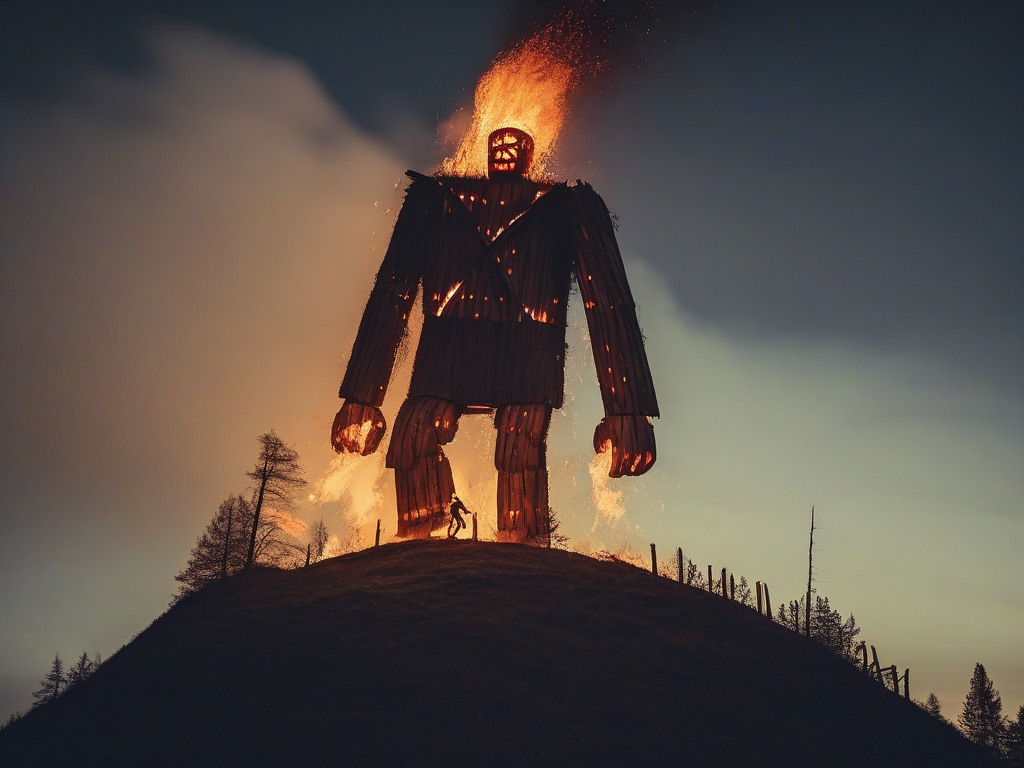
\includegraphics[width=\columnwidth]{img/scirpex-hill.jpg}
\end{center}
Golem creati tramite il sacrificio di 8-10 legionari della Legio IX scomparsa.
%
Vedi pagina 174 del manuale Britannia~\cite{britannia_en} per maggiori informazioni.
}

I custodes possono scegliere se ingaggiarlo con armi a distanza, o ordinare agli ausiliari di istanza nel castrum di attaccare con archi lunghi.
Qualora tentassero di ingaggiare in mischia, malcapitati passanti o ausiliari in fuga tenteranno di dissuaderli.

Il gigante muove solo pochi passi prima di accasciarsi a terra, ormai lontano dallo sguardo del druido che lo controlla, e lentamente soccombe all'incendio che ne divora il corpo.
Sembra che all'interno dei giunchi ci sia qualcosa, ma non si capisce bene cosa.

L'incendio distrugge il patibolo dove l'esecuzione di Georgius sarebbe dovuta avvenire e i custodes saranno chiamati a prioritizzare le indagini o l'esecuzione di un condannato politicamente scomodo.

%%%%%%%%%%%%%%%%%%%%%%%%%%%%%%%%%%%%%%%%%%%%%%%%%%%%%%%%%%%%%%%%%%%%%%%%%%%%%%%
\section*{Parte II -- Eco dal Passato}
%
\subsection*{Scena VII\\Ritrovamenti}

Sul campo di battaglia vengono rinvenuti i corpi di tre legionari romani.
Uno di loro \`{e} gi\`{a} morto. Per gli altri due servir\`{a} un intervento immediato per curare le loro ferite per salvargli la vita (\tiro{De Scientia (Medicina)}{6}).
Nel caso venisse salvata loro la vita, i legionari saranno incoscienti per 24 ore, e intontiti per un altro giorno.
Dal campo di battaglia riemerge anche un altro ferito, che i custodes pi\`{u} attenti (\tiro{Sensibilitas}{6}) riusciranno solo a intravedere di sfuggita prima che si dilegui nella nebbia.
Si tratta dell'antico Arcibardo, che si reca a cercare rifugio presso le abitazioni circostanti.

\object{Aquila della Legio IX}{
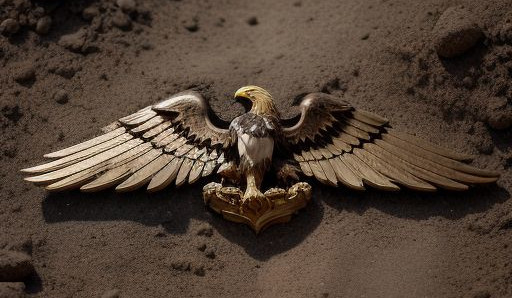
\includegraphics[width=\columnwidth]{img/vessillo.jpeg}
Dalla terra riemergono solo resti bruciacchiati di questo vessillo, in origine applicato sulla cima di uno stendardo.
Sulle ali dell'aquila viene riportata l'incisione \textsc{IX Hispana}.

\emph{+3 a tutti i tiri di \textbf{De Bello} e +6 a tutti i tiri \textbf{Auctoritas}} a tutti i legionari romani durante il combattimento. Il legionario deve vedere il vessillo. L'effetto si applica anche ai custodes.
}

Dai resti dello scirpex, riemergono i cadaveri inceneriti di 10 legionari romani, riconoscibili dal metallo della loro lorica segmentata.
Un \tiro{De Scientia (Indagare)}{9} rivela ai custodes la presenza di un vessillo in oro massiccio a forma di aquila.
%
Un \tiro{De Scientia (Storia)}{3} rivela ai custodes le seguenti informazioni:

\emph{I grado di successo:}\\
Il vessillo dell'aquila viene usato solo in occasione di grandi battaglie e infonde coraggio e forza ai legionari durante la battaglia.
Pochi sono i casi registrati di perdita del vessillo in battaglia.
Intere legioni hanno combattuto fino alla morte con il solo scopo di recuperare un'aquila romana caduta in mano nemica.

\emph{II grado di successo:}\\
Il vessillo della Legio IX scomparve oltre 350 anni fa da Eburacum senza lasciare traccia.
Si teme sia stato perso durante una rivolta delle trib\`{u} del nord in cui la legione intera venne sconfitta.

\emph{III grado di successo:}\\
Successive spedizioni di ricerca non trovarono cadaveri n\`{e} tracce di battaglia e la fine di questa legione e del suo vessillo rimase avvolta nel mistero.
Se portato sul campo di battaglia, esso conferisce ai legionari sotto la sua ombra grandi poteri di combattimento.


\subsection*{Scena IX\\Presagi Funesti}
%
Nelle ore che seguono, piccole scosse di terremoto si susseguono.
Corvi volano il cerchio in cima alla collina.
Altri omen di sventura fanno presagire un pericolo imminente.

Nel caso in cui i custodes non li abbiano notati dopo la battaglia, il giorno dopo una squadra di ricognizione trover\`{a} i due legionari feriti.

I custodes possono indagare per scoprire maggiori informazioni nei successivi giorni.
Quando i legionari feriti si riprendono, chiederanno udienza immediata con Quinto Petilio Ceriale per fare rapporto sulla minaccia che stavano combattendo e allertare con urgenza l'imperatore Adriano.

I legionari feriti sono ignari del tempo trascorso.
Per loro il combattimento \`{e} iniziato un giorno fa, ma nell'impero sono trascorsi pi\`{u} di 350 anni.
Costoro non sono al corrente della costruzione del Vallo di Adriano, n\`{e} tantomeno della Lex Arcana approvata dal Senato sotto la guida dell'Imperatore Teodomiro.

I legionari riferiranno di aver visto i loro compagni venire accerchiati da un'imboscata sulla collina.
Molti sono caduti in trappole tese dai druidi, i quali hanno sacrificato prigionieri romani per evocare giganti che non sanguinano.
Loro si sono lanciati all'assalto di uno di questi giganti seguendo l'aquila della legione.
Sono riusciti ad incendiarlo ma non ad abbatterlo (\`{e} stato consumato dalle fiamme mentre loro erano svenuti).

\monster{Vate}{
\dvstat{6}
{De Corpore, Sensibilitas}
{De Bello, De Natura, De Societate, Punti Vita}
{De Magia (Disciplina Druidica)}
{12}
\equip{Sica (Danno 4)}{Nessuna}
\specialstat{-}{Tiro del Fato}
}

I legionari riferiranno inoltre di stare combattendo contro un esercito coalizzato di Picti, Briganti, ed anche Hiberni che contava diverse centinaia di uomini.
La legio IX raramente aveva affrontato un esercito cos\`{i} numeroso, ma il problema sono i giganti che fanno strage tra i ranghi romani.
Riferiranno di avere visto ancora \textbf{1:1} giganti che ancora combattono contro i legionari.
Ciascuno di questi \`{e} controllato a vista da un vate.

\subsection*{Scena X\\Musica di Altri Tempi}
%
Il musico bicentenario passa per caso dalla taverna del villaggio, fa il suo spettacolo, ma quando capisce che qualcosa di funesto sta per accadere, decide di lasciare Pons Aelium in cerca di locande meno pericolose.
I custodes possono provare a fermarlo, ma dovranno essere molto convincenti (\tiro{De Societate}{9} oppure tramite 5 successi in una Udienza a difficolt\`{a} 6).
Se i custodes lo arrestano o lo minacciano, egli non oppone resistenza, ma si rifiuter\`{a} di aiutare Roma in qualunque modo.

Nel caso in cui non sia gi\`{a} stato introdotto al seguito del contubernium, Ellfin Pupius raggiunge i custodes per chiedere aggiornamenti riguardo le loro indagini e offrir\`{a} collaborazione per indagare.

Dopo essersi ripreso dalle ferite in un nascondiglio segreto poco lontano, l'antico arcibardo Cluas a' Ge\`{a}rra si fa trovare da Pupius e chiede un incontro coi custodes.
Cluas non parla bene latino, e chiede l'intervento di Pupius come interprete.
Cluas si accinge a guidare i custodes verso il luogo dove il rituale per manipolare lo spazio-tempo venne officiato, nella miniera di antimonio.
Tuttavia, negli anni i tunnel sono crollati e ora servono dai 3 ai 5 giorni di lavoro per riaprire il passaggio.

Brevi indagini sul sito rivelano che i lavori di livellamento del terreno in cima alla collina hanno causato smottamenti nelle miniere che hanno disturbato il rituale druidico.

Cluas racconta di non essere stato lui ad officiare il rituale, bens\`{i} Sp\`{o}g Nan Sionnach, il quale si trova ancora nel reame fatato.
Solo Sp\`{o}g \`{e} capace di una magia cos\`{i} potente, mentre Cluas pu\`{o} al massimo prolungare di alcune ore o al massimo dei giorno l'effetto della magia.
Questa azione richiede di trovare, e posizionare nella miniera altre ghiande magiche.
Al contrario, se i custodes lo desiderano, l'arcibardo \`{e} in grado di terminare la magia immediatamente e riportare legionari, barbari, e scirpex nel mondo attuale.

\object{Ghiande Magiche}{
\begin{center}
\vspace{-1em}
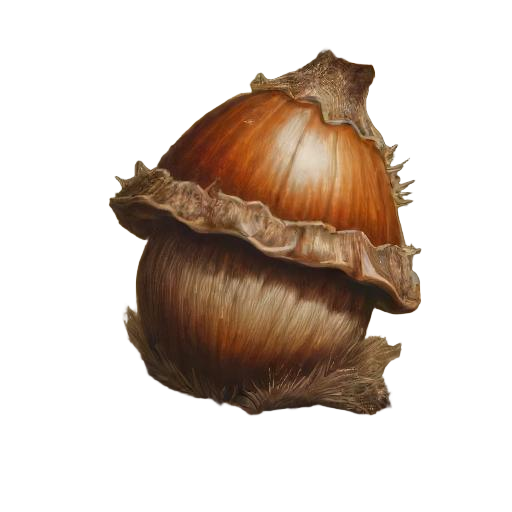
\includegraphics[width=.3\columnwidth]{img/ghianda.png}
\vspace{-2em}
\end{center}
Si tratta di ghiande sacre per i druidi e si raccolgono sotto le querce di Britannia e Hibernia.
Non tutte hanno lo stesso potere magico.
I loro effetti si possono leggere nella Tabella a pagina 118 del manuale Britannia~\cite{britannia_en}.
}

%%%%%%%%%%%%%%%%%%%%%%%%%%%%%%%%%%%%%%%%%%%%%%%%%%%%%%%%%%%%%%%%%%%%%%%%%%%%%%%
\section*{Parte III -- La Battaglia pi\`{u} Lunga}
%
\subsection*{Scena XI\\Vecchi Nemici}
%
Le voci corrono in fretta e -- non si sa come -- hanno raggiunto anche altre trib\`{u} oltre il Vallo.
Un esercito di fanatici dormienti di Balor attacca il Segedunum, un forte a est di Pons Aelium, mentre un manipolo di questi prova ad aggirare il Vallo via fiume.
Due dozzine di invasori riescono ad approdare e si dirigono verso il villaggio di Pons Aelium.
Un messaggero giunge lungo il vallo e porta notizia dell'attacco chiedendo rinforzi.
Il capo della guardia decide di mantenere il minimo indispensabile (una decina) di legionari a Pons Aelium e invia i restanti come rinforzi a Segedunum.

Poco dopo la partenza dei rinforzi, un piccolo distaccamento dell'esercito invasore si avvicina alla collina.
Allertati da un minatore, i custodes sono chiamati a difendere gli scavi per liberare i cunicoli.

\monster{Pitto Fanatico}{
\dvstat{5}
{Ratio, Sensibilitas}
{De Corpore, De Natura, Vigor}
{De Bello, Punti Vita}
{15}
\equip{Spada Celtica (Danno 8), Arco (Danno 6)}{-}
\specialstat{Carica\footnote{+1 grado di successo al moltiplicatore danno durante il primo tempus di attacco. Vedi manuale Corebook~\cite{corebook_en} a pagina 138.},
Assetato di Sangue\footnote{+1 al moltiplicatore di danno in combattimento corpo a corpo, sia in attacco sia in difesa. Vedi manuale Dacia e Tracia~\cite{dacia_tracia_en} a pagina 108.},
Tattiche del Branco\footnote{+1DV a De Corpore e De Bello se 2 o pi\`{u} NPC sono ingaggiati in corpo a corpo contro lo stesso nemico. Vedi manuale Corebook~\cite{corebook_en} a pagina 139.}}
{--}
}

Gli attaccanti sono in numero \textbf{1:1} pitti fanatici + 1 vate.
Nel caso in cui i custodes portino rinforzi, \textbf{1:2} fanatici (un fanatico ogni ausiliari di rinforzo) possono bilanciare lo scontro.
Non \`{e} comunque possibile richiedere l'aiuto di pi\`{u} di 3 ausiliari per non lasciare sguarnito il castrum.

\subsection*{Scena XII\\Il Giuramento}
%
Al termine dello scontro, i custodes avvertono la sensazione di pericolo sempre pi\`{u} imminente.
Omen e presagi di catastrofi in avvicinamento si moltiplicano.
Uno dei custodes riceve in sogno la visione delle divinit\`{a} vallo (vedi box \emph{Le Guerriere del Vallo}), gli altri avvertiranno generici presagi di un alleato a ovest che li attende, e nemici ad est in avvicinamento.
%
\dream{Le Guerriere del Vallo}{
Un ruscello scorre sereno.
Sulla riva opposta, una siepe sta fiorendo.
All'improvviso, lo scheletro di un cavallo dagli occhi infuocati scavalca la siepe dirigendosi verso il ruscello e lo oltrepassa per poi mutare forma e trasformarsi in tanti serpenti.
Mentre la creatura salta, i fiori appassiscono, la siepe deperisce e un gruppo di bambini che giocano lungo il ruscello iniziano a piangere.
\emph{I bambini sono in numero pari ai custodes + 4.}
Dalla sinistra, compaiono quattro corvi.
Questi pare che escano da un nido posto nella siepe, volano in cerchio e poi si posano su 4 bambine che piangono.
Le bambine smettono immediatamente di piangere e iniziano ad accarezzare i corvi.
Rasserenate dagli uccelli, iniziano ad aiutare gli altri.
Una imbraccia un pezzo di legno e lo usa per bloccare il morso di un serpente.
La seconda usa un pugnale per liberare un altro bambino dalla morsa di un altro serpente.
La terza incoraggia vivacemente gli altri bambini e sgrida chi cerca di scappare, mentre la quarta si scaglia contro il nido di serpenti urlando.
}
Interpretare questo sogno porta le seguenti informazioni:

\emph{I grado di successo}:\\
Il vallo non \`{e} solo sassi e fango, bens\`{i} brulica di vita (fiori).
Quando forze soprannaturali minacciano i pi\`{u} deboli, dai dintorni del vallo, forze altrettanto potenti ascoltano il loro pianto e accorrono in loro soccorso.

\emph{II grado di successo}:\\
Da ovest, una o pi\`{u} divinit\`{a} guerriere sono pronte ad intervenire per aiutare gli indifesi e riequilibrare le sorti di una battaglia ingiusta.
I figli e le figlie del Vallo conoscono questo culto e trovano forza e ispirazione in questa presenza.

\emph{III grado di successo}:\\
Queste quattro divinit\`{a} hanno genere femminile e non appartengono al pantheon ufficiale, tuttavia non sono ostili a Roma.
In generale, hanno il potere di incitare, proteggere, punire, e liberare chi combatte per una giusta causa.
Nello specifico, ciascuna ha un suo potere ed un suo strumento distintivo, ma agiscono spesso insieme.
Al cospetto del loro altare (nido) si pu\`{o} invocare il loro intervento.

Un \tiro{De Magia (Culti Imperiali)}{9} rivela l'identit\`{a} di queste divinit\`{a}: le dee \emph{Alaisiagae}\footnote{Vedi manuale Britannia~\cite{britannia_en} a pagina 103.} che hanno un altare consacrato a loro presso il tempio di Marte di Vercovicium.
Si chiamano Baudihilla ``signora della battaglia'', Beda ``la protettrice'', Fimmilena ``la vendicatrice'', e Friagabis ``che concede la libert\`{a}''.
Il grado di difficolt\`{a} scende a 6 nel caso in cui il custos sia originario della provincia di Britannia o sia un guerriero.
Un guerriero originario della Britannia avr\`{a} grado di diffolt\`{a} 3.

Lungo il viaggio verso Vercovicium, i custodes incontrano Publius Aurelianus Constans, il quale racconta di attacchi diffusi e scoordinati lungo tutto il vallo dal parte di fanatici religiosi di culti ormai dati per estinti.
Nessuno di questi costituisce reale pericolo, ma il tempismo impressiona tutti.
Grazie alla sua rete di informatori e alle sue abilit\`{a} di tattica militare, sta spostando rinforzi lungo il vallo dove prevede che arriveranno i prossimi assalti.

Il viaggio dura 12 h di marcia, e una volta arrivati i custodes possono recarsi a pregare al tempio di Marte.
Pregare o lasciare una offerta all'altare di Marte porta i seguenti benefici.
\begin{table}[h]
\begin{tabular}{| m {.55\columnwidth} | >{\raggedleft\arraybackslash} p {.35\columnwidth} | }
\hline
Custos	 		&	+ 1d3 pietas \\
\hline
Custos con dono 	&	+ 1d6 pietas \\
\hline
Guerriero 		&	3 + 1d3 pietas \\
\hline
Guerriero con dono	&	3 + 1d6 pietas \\
\hline
\end{tabular}
\end{table}

Pregare o lasciare una offerta all'altare delle Alaisiagae scatena un evento portentoso.
Le porte del tempio si spalancano di colpo ed una folata di vento entra improvvisamente.
Un tornato di sabbia e di foglie si avvolge attorno al contubernium per poi placarsi e lasciare un cerchio perfetto di fiori, foglie secche e piume di corvo attorno a due delle quattro statue accanto all'altare.
Un sacerdote si fa avanti, stupito ma orgoglioso.

Sacerdote --
\say{%
Avete attirato l'attenzione delle dee Alaisiagae.
Non accade quasi mai che siano le dee a farsi avanti per prime, da anni non vedevo un evento simile.
Vi stanno offrendo la loro investitura.
Se decidete di accettare, sar\`{a} mia gioia officiare il rituale}

Se i custodes chiedono maggiori informazioni, il sacerdote continua

-- \say{%
Beda e Fimmilena sono dalla vostra parte.
Vi offrono il loro potere, se giurate di usarlo per difendere i pi\`{u} deboli e proteggerli dagli oppressori.}

Se i custodes rifiutano, il sacerdote si ritira offeso e non accade altro degno di nota.
Se invece accettano, il rituale dura una decina di minuti, durante i quali viene disegnato il simbolo di un corvo su scudo e armatura di tutti i custodes, e vengono decorati da una collana di corda e fiori.

-- \say{%
La collana vi tiene legati al vostro giuramento, il corvo vi difende dagli aggressori, la vostra volont\`{a} e la vostra forza vi faranno da guida fino a che non avrete vinto questa battaglia!}

I custodes beneficiano dei seguenti effetti fino alla fine dell'avventura. Non \`{e} possibile rimuoverli.
Un \tiro{De Magia}{9} rivela ai custodes la natura di questi bonus.
In caso di fallimento, i bonus si manifesteranno alla prima azione rilevante.
\begin{description}
\item[Benedizione di Beda] +3 parata a tutti gli scudi, +1 protezione a tutte le armature
\item[Maledizione di Fimmilena] 1d6 danno ogni volta che il custos infrange il giuramento
\end{description}


\subsection*{Scena XIII\\Un Impiccato in Sospeso}
%
\monster{Delegato Brigante}{
\dvstat{6}
{Ratio}
{De Bello, De Corpore, De Natura, Sensibilitas}
{Punti Vita}
{18}
\equip{Lancia (Danno 6), Spada Celtica (Danno 8), Arco (Danno 6)}{Clipeus (Parata +2)}
}

Prima di avviarsi verso la collina per interrompere la magia druidica, i custodes saranno chiamati a pronunciarsi sul destino di Georgius ancora tenuto in custodia.
La delegazione di briganti sollecita il rilascio di Georgius.
Hanno la sensazione che il castrum abbia meno legionari di guardia del solito e potrebbero organizzare un assalto per liberare il giovane.

I custodes possono negoziare con i briganti per il rilascio di Georgius.
Un \tiro{De Societate (Negoziare)}{6} porta i seguenti risultati.
Il grado di difficolt\`{a} scende a 3 se i custodes portano dei doni o si offrono di intercedere per liberare Georgius.

\emph{I grado di successo}:\\
I briganti non assaltano il forte e si ritirano immediatamente con Georgius.

\emph{II grado di successo}:\\
I briganti ripagano i danni causati da Georgius e porgono scuse ufficiali.

\emph{III grado di successo}:\\
I briganti forniranno aiuto militare ai custodes per difendere il Vallo nei giorni a seguire in cambio della libert\`{a} di Georgius.

Se i negoziati falliscono o i custodes non si accordano a questi termini, ci sono \textbf{2:1} guerrieri briganti che -- forti della superiorit\`{a} numerica rispetto ai custodes -- sono pronti a fare irruzione nel castrum.

\subsection*{Scena XIV\\Magia Fomoriana}
%
Dopo giorni di estenuanti lavori, i tunnel per accedere alla vecchia miniera di stibium sono stati liberati.
L'arcibardo \`{e} pronto a mantenere il rituale in modo pi\`{u} stabile o interromperlo definitivamente, seguendo le indicazioni dei custodes.

All'interruzione del rituale, il cielo si colora di grigio e un odore di acre di cadaveri bruciati si permea l'aria sulla collina.
Urla di guerra in lingue celte ed in latino si odono da miglia di distanza.

\monster{Antico Guerriero Ribelle}{
\dvstat{6}
{Ratio, Sensibilitas}
{De Natura, De Bello, Vigor, Punti Vita}
{De Corpore}
{12}
\equip{Spada Celtica (Danno 8)}{Clipeus (Parata +2)}
}

Un esercito di circa 500 guerrieri pitti, caledoni, iberni, e briganti compare dal fumo.
Dietro di loro, \textbf{1:1} vati comandano altrettanti scirpex alti 8 piedi ciascuno.

Migliaia di legionari romani faticano a mantenere la formazione di fronte agli attacchi degli scirpex.
Nonostante la superiorit\`{a} numerica, l'intera Legio IX non riesce a fare breccia tra le linee nemiche e anzi effettua spesso brevi ritirate strategiche.
Ora l'intera collina \`{e} un campo di battaglia.

Ogni due tempora, un manipolo di legionari scompare dalla vista, probabilmente in un buco nel terreno.
Superando un \tiro{Ingenium}{6}, ad un custos appare evidente che i vates hanno disseminato trappole lungo il fronte per catturare vivi dei legionari e usarli come sacrifici.
Una di queste trappole sembra essere particolarmente grande, un buco nelle linee imperiali si \`{e} appena formato e i ribelli spingono per avanzare.

\monster{Emissario di Balor}{
\emph{Dimensione: 5}
\begin{center}

\includegraphics[width=.75\columnwidth]{img/balor.jpeg}
\end{center}
\dvstat{20}
{Danno, De Corpore}
{-}
{-}
{6000}
\emph{De Bello di questa creatura \`{e} pari a 600.}\\
\specialstat{Afferrare}{Terrore (1 DV, la vittima deve vedere la creatura)}%
Scirpex ottenuto sacrificando circa 50 legionari romani.
Non \`{e} possibile incendiarlo.
L'arcivate controlla questa bestia.
}

Da questo buco, si erge una figura mastodontica, seguita soltanto da un uomo.
Un golem alto 40 piedi si erge maestoso sulla collina.
Purtroppo, non \`{e} amico di Roma.
Uno dei PNG vicino ai custodes riconosce Balor, portatore di distruzione dei Fomoriani, che non pu\`{o} essere stato evocato che dall'Arcivate.
Un \tiro{Sensibilitas}{6} oppure un \tiro{De Magia (Culti Proibiti)}{9} sono sufficienti per capire che non si tratta dell'incarnazione di una divinit\`{a}, bens\`{i} di una creatura inanimata ma non meno pericolosa.
L'emissario di Balor \`{e} uno scirpex ottenuto sacrificando 50 legionari romani ed \`{e} immune al fuoco.

\monster{Arcivate}{
\dvstat{10}
{De Corpore, Sensibilitas}
{De Bello, De Natura, De Societate, Punti Vita}
{De Magia (Disciplina Druidica)}
{20}
\equip{Sica (Danno 4)}{-}
\specialstat{-}{Tiro del Fato}
\begin{center}
\vspace{-1.5em}

\includegraphics[width=.75\columnwidth]{img/arcivate.jpeg}
\end{center}
}

I custodes hanno 5 tempora per agire prima della comparsa delle dee Alaisiagae.

\subsection*{Scena XV\\Un Destino Sospeso nel Tempo}
%
Quattro carri da guerra appaiono sulla collina.
Ciascuno di essi \`{e} trainato da una fanciulla.
Si muovono con velocit\`{a} innaturale e si uniscono alla battaglia.
Una volta per tempus, si applicano i seguenti effetti.
\begin{description}
\item[Carro di Baudihilla] Baudihila si lancia alla carica con la sua spada alata. Uccide un nemico sul colpo, ma cerca di farsi strada per distruggere i nemici pi\`{u} pericolosi. 25\% possibilit\`{a} che uccida un vate che sta controllando uno scirpex.
\item[Carro di Beda] Mentre un custos o un legionario sta per ricevere un colpo, Beda interviene deviando il colpo con il suo scudo.
\item[Carro di Frigiabis] Taglia la gola ad un vate che sta per sacrificare altri 10 legionari e li libera.
\item[Carro di Fimmilena] Raduna le unit\`{a} romane in fuga. Il suo colpo di frusta le spinge a riprendere la formazione.
\end{description}

Alla morte di un vate, lo scirpex corrispondente smette di muoversi il tempus successivo, e si accascia a terra nei successivi 2 tempora.

Per arrivare in vista dell'arcivate (distanza lunga o distanza media), i custodes devono difendersi da schermaglie di \textbf{1:1} guerrieri ribelli.

Per arrivare in corpo a corpo con l'arcivate, i custodes devono ingaggiare un cordone difensivo di guerrieri ribelli. Per fare breccia tra le linee difensive, i custodes devono neutralizzare 3 ribelli in prima linea + \textbf{1:1} rinforzi nelle retrovie.

Alla morte di tutti i vates e dell'Arcivate, la Legio IX Hispana riesce a respingere i ribelli nel giro di poche decine di minuti.
Quest'oggi i canti di vittoria saranno in latino.

\section*{Conclusione}
%
L'arcidruido viene trovato senza vita alla fine della battaglia.
Il suo amico arcibardo gli rende onore e vi chiede il permesso di allestire una pira secondo tradizione celtica.

Marte si rallegra che lo scontro si \`{e} combattuto e questa battaglia ha consacrato a lui l'intera collina.
La storia di questa battaglia si narrer\`{a} molto pi\`{u} a lungo di quanto le mura di un tempio possano reggere.
I lavori di costruzione possono riprendere, dopo che la terra avr\`{a} assorbito tutto il sangue ribelle.

La legione perduta \`{e} stata ritrovata.
I libri di storia devono essere riscritti poich\'{e} quello che finora si pensava fosse una terribile sconfitta per Roma \`{e} stata oggi trasformata in una vittoria in quella che molto probabilmente verr\`{a} ricordata come la battaglia pi\`{u} lunga della storia dell'impero.

Nonostante le perdite, ora la Britannia si ritrova con un enorme surplus di personale militare.
Una volta terminata la reintegrazione dei veterani nella societ\`{a} moderna, Roma avr\`{a} le forze necessarie per tornare ad occupare il Vallo Antonino o perfino per completare la conquista dell'isola.
L'imperatore sapr\`{a} decidere con saggezza.

\subsection*{Punti Esperienza}
\begin{description}
\item[+6] Valore base
\item[+1] I custodes risolvono il mistero della birra marcia
\item[+1] I custodes intercedono per evitare l'impiccagione di Georgius
\item[+2] I custodes restaurano e portano in battaglia il vessillo della Legio IX, ristabilendo il suo onore
\end{description}

\section*{Riconoscimenti}
Le immagini sono state tutte generate automaticamente tramite \emph{AI Image Generator} disponibile da \url{deepai.org}.

%%%%%%%%%%%%%%%%%%%%%%%%%%%%%%%%%%%%%%%%%%%%%%%%%%%%%%%%%%%%%%%%%%%%%%%%%%%%%%%
\bibliographystyle{unsrt}
\bibliography{references}
\end{document}
